% tex file for regression

\par \indent A simple and straightforward way to model the voxel time courses 
for each subject is to perform linear regression. Initially, we just used the 
convolved predicted hemodyamic response (HR) and either all the of the 
conditions together or each of conditions individually. After realizing that 
the HRs themselves didn't explain enough of the BOLD ratio, we attempted to 
add features in order to reduce or explain the noise we observed. Additional 
features that we examined included a linear drift and some of the time 
courses' Fourier series and principal components.

\par Linear regression assumes a linear relationship between a response 
vector $y$ and a design matrix of predictors $X$. Each element of $y$ 
represents a single observed response, and each row of $X$ represents a 
corresponding vector of predictor values. If including the intercept as a 
term (as we have elected to do), the first column of the $X$ design matrix 
should be a vector of $1$s. The linear model can then be expressed as: 

\begin{equation}
y = X\beta + \epsilon
\end{equation}

\par It is further assumed that the errors $\epsilon_i$ for each observation 
$i$ are independent and identically distributed with $N(0, \sigma^2)$, and 
that the errors are independent of $X$. The vector of coefficients $\beta$ 
with length equal to the number of predictors in $X$ can be estimated with 
the closed-form solution:

\begin{equation}
\hat{\beta} =(X^T X)^{-1} y
\end{equation}

\par In our case, we actually want to fit a linear model to each individual 
voxel's time course. Matrix algebra provides a convenient solution. Instead of 
considering the time course for each voxel individually as a single $y$ 
vector, we can instead consider the voxel $\times$ time matrix $Y$. Our model 
is then:

\begin{equation}
Y = X\beta + \epsilon
\end{equation}

\noindent and our $\beta$ estimates are then also a matrix: 

\begin{equation}
\hat{\beta} =(X^T X)^{-1} Y^T
\end{equation}

\par Even when $(X^T X)$ is not invertible, $\hat{\beta}$ can be estimated 
using the pseudo-inverse of $(X^T X)$, represented as $(X^T X)^{-}$ to get a 
non-unique value for $\hat{\beta}$.

\par To consider the strength of the effects of these predictors, we will use 
t-tests of the corresponding estimated coefficients for each voxel and 
subject, as discussed under \textit{"Hypothesis Testing"}. The validity of the 
model and of the ``p-values'' produced by performing these t-tests is 
dependent on whether or not the many assumptions of the linear model are 
actually met. In particular, we will discuss the assumption of normal errors 
by analyzing the residuals in the \textit{"Normality Assumptions"} section. 

\subsubsection{More about potential features:}
\par Other than the basic HR feature/features and a column of $1$s (to account 
for an ``intercept'' term or non-zero average value), we experimented with 
including additional predictors in our design matrix $X$. Among these were the 
first few principal components of the voxel $\times$ time matrix of voxel time 
courses and the first few functions of the Fourier series for the time courses. 
As noted above these, additional features helped account for the noise in the 
observed BOLD ratio fluctuation.

\vspace{2mm}
\noindent \textbf{Principle Components}
\vspace{2mm}
\par One approach for reducing the noise in the linear model is to include 
principal components of the voxel $\times$ time voxel time course matrix. 
Instead of using the entire matrix, it may be possible to just include the 
first few principal components as features that explain a great deal of the 
variance in the entire matrix. To get the principal components, we obtained 
the singular value decomposition (SVD) of the time $\time$ time covariance 
matrix. We tried this with and without first masking the voxels. To 
standardize the voxels, we subtracted the column means (mean across voxels) 
from the voxel by time matrix. There is also a very strong effect of mean 
over time in the data that dominates other effects, so we subtracted the 
row means (mean over time) as well.

As you can see in Figure \ref{fig:pca10}, which compares the variance 
explained by including up to ten components, with and without masking the 
voxels, masking explains more variance at each component. This trend was 
observed across all subjects. So, between the better performance and the 
logical rationality of using the masked data (we are not actually interested 
in the behvavior of voxels outside the brain), we decided to only work with 
the masked data's principal components. 

\begin{figure}[ht]
	\centering
	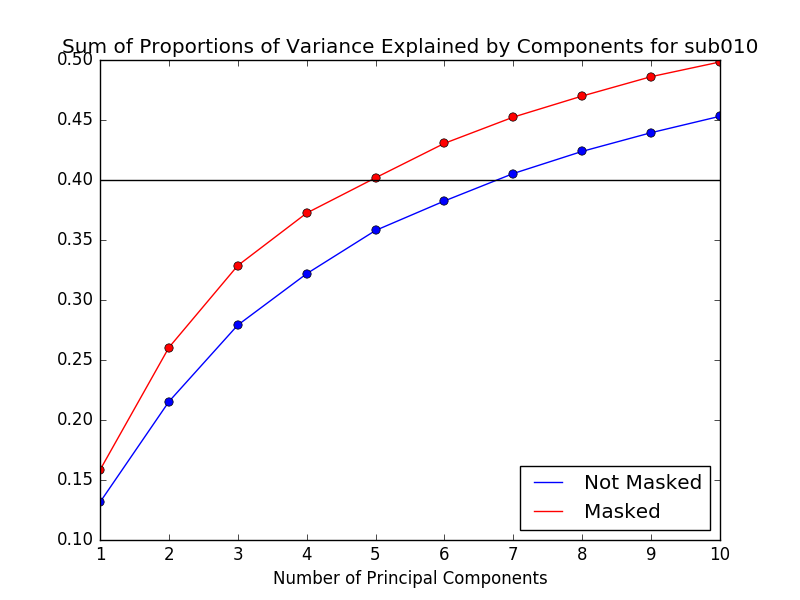
\includegraphics[width=.5\linewidth]{../images/pcacumsumssub010.png}
 	\caption{Comparing proportion of variance explained by Subject 10's 
principal components, with and without masking the data.}
 	\label{fig:pca10}
\end{figure}

An important issue to consider is how many principal components to include in 
the design matrix. Figure \ref{fig:pcabox} compares the the amount of variance 
explained by including successively more principal components across subjects. 
A few observations should be noted. First, there is considerable variation 
between subjects in how much variance the early principal components capture. 
Second, by including only the first six components, it is possible for each 
subject's voxel time course matrix to capture at least 40\% of the variance. 
Moving forward, we chose to include six principal components as additional 
features when considering models that reduce noise. This cutoff of six 
components or 40\% of the variance explained was somewhat arbitrary, with the 
idea being we wanted to only include a few components without sacrificing too 
much of the variance explained and that we wanted to use the same number of 
components for each subject. It will be seen later that the variation between 
subjects in how much variance is captured by the first six components has strong 
ramifications on the results. 

\begin{figure}[ht]
	\centering
	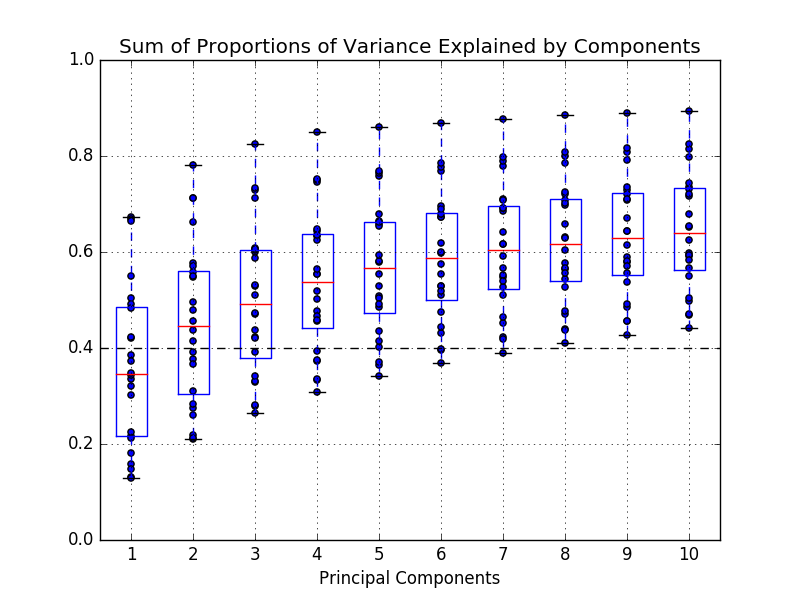
\includegraphics[width=.5\linewidth]{../images/pcaBOX.png}
 	\caption{Boxplots comparing the amount of variance captured by principal 
components for each subject. The data was masked beforehand. All subjects are 
able to capture at least 40\% of the variance when using just six principal 
components.}
 	\label{fig:pcabox}
\end{figure}


\vspace{2mm}
\noindent \textbf{Fourier Series}
\vspace{2mm}
\par We included 4 features related to the first few functions of the Fourier series.
The full fourier series is represent as the following:

\begin{equation}
f(x) = \frac{1}{2} \cdot a_0 + \sum_{n=1}^{\infty} a_n \cdot cos(n x) + \sum_{n=1}^{\infty} b_n \cdot  sin(n x)
\end{equation}

\noindent but since strength of Fourier series strength comes from 
orthogonality of the range, and we are looking for a function of the range 
$(0, \text{num of TR})$, we change it to:

\begin{equation}
f(x) = \frac{1}{2} \cdot a_0 + \sum_{n=1}^{\infty} a_n \cdot cos(\frac{n}{\text{num of TR}} x) + \sum_{n=1}^{\infty} b_n \cdot sin(\frac{n}{\text{num of TR}} x)
\end{equation}

\noindent We used $ + \sum_{n=1}^{2} a_n \cdot cos(\frac{n}{\text{num of TR}} x) + 
\sum_{n=1}^{2} b_n \cdot sin(\frac{n}{\text{num of TR}} x)$ to be 4 features to try 
to get a low order sinusoidal fluxucations.

\subsection{Model Selection}

\par In order to select the best set of features for our $X$ matrix, and also 
compare the use of a single condition feature vs. each of the 3 different types
of conditions as 3 seperate features, we decided to utilize model comparison; 
specificially, AIC, BIC, and Adjusted $R^2$ metrics. Using small expressive
subset of the subjects ($002$,$003$, and $014$) we abused the metric's by
averaging across all voxels and people.  We visualized values in the Figures
\ref{fig:AIC},\ref{fig:BIC}, and \ref{fig:adjr2}.

\par From these plots, you can observe that we don't gain much from adding
the conditions seperated, and from the BIC, we decided that the Fourier
features didn't add enough benefit and justify the increase of features. Thus, 
we'll be using the model that includes a single HRF for all the conditions, 
a linear drift feature, and the first 6 principle components. It is possible 
that this will dangerously overfit, and even with these features we could have
overfit beyond just the noise and into the territory of the hemodyamic 
response.

%\begin{table}
%\centering
%	\begin{tabular}{l ||  l   |  l  |   l    | l  | l  |  l}
%X value & 1 &        2       &             3       &     4         &        5        &         6       \\
%	 \hline
%	 & HRF &   HRF       &  HRF            & HRF         &  HRF        & HRF  \\
%	 &        &   + DRIFT &  + DRIFT      & + DRIFT  &  + DRIFT   & + DRIFT  \\
%	 &        &                 &  + FOURIER &  + PCA 4 &  + PCA 6   & + FOURIER \\
%	 &        &                 &                      &                &                   & +  PCA 6 \\
%	
%
%	\end{tabular}
%\caption{Explaining Plot X values}
%\label{tab:plot}
%\end{table}


%\begin{table}
%
%\begin{minipage}[b]{1\linewidth}
%	\centering
%	\scriptsize{\begin{tabular}{l ||   l  |  l  | l  | l  |l   |  l}
%	 & HRF &   HRF     &  HRF       & HRF      &  HRF       & HRF  \\
%	 &     &   + DRIFT &  + DRIFT   & + DRIFT  &  + DRIFT   & + DRIFT  \\
%	 &     &           &  + FOURIER &  + PCA 4 &  + PCA 6   & + FOURIER \\
%	 &     &           &            &          &            & +  PCA 6 \\
%	\hline
%	All conditions together   &  589.313 &  503.388 &  452.366 & 337.296 & 288.452 &   266.126 \\
%	All conditions seperately & 587.824 &  501.184 &  449.337 &   331.995 & 286.85 &   264.756 \\
%	\end{tabular}}
%	\label{tab:AIC}
%	\center{\caption{AIC}}
%\end{minipage}	
%
%\begin{minipage}[b]{1\linewidth}
%	\centering
%	\scriptsize{\begin{tabular}{l ||   l  |  l  | l  | l  |l   |  l}
%	 & HRF &   HRF     &  HRF       & HRF      &  HRF       & HRF  \\
%	 &     &   + DRIFT &  + DRIFT   & + DRIFT  &  + DRIFT   & + DRIFT  \\
%	 &     &           &  + FOURIER &  + PCA 4 &  + PCA 6   & + FOURIER \\
%	 &     &           &            &          &            & +  PCA 6 \\
%	\hline
%	All conditions together    &  596.409 &  514.032 &  477.202 &    365.68 &316.835&  308.702\\
%	All conditions seperately & 602.016 &  518.924 &  481.269  360.379 & &  322.33 & 314.427 \\
%	\end{tabular}}
%	\label{tab:BIC}
%	\caption{BIC}
%\end{minipage}	
%
%
%\begin{minipage}[b]{1\linewidth}
%	\centering
%	\scriptsize{\begin{tabular}{l ||   l  |  l  | l  | l  |l   |  l}
%	 & HRF &   HRF     &  HRF       & HRF      &  HRF       & HRF  \\
%	 &     &   + DRIFT &  + DRIFT   & + DRIFT  &  + DRIFT   & + DRIFT  \\
%	 &     &           &  + FOURIER &  + PCA 4 &  + PCA 6   & + FOURIER \\
%	 &     &           &            &          &            & +  PCA 6 \\
%	\hline
%	All conditions together    & 0.007  &  0.198  &  0.323  &  0.527   &  0.596  & 0.631 \\
%	All conditions seperately & 0.02   &  0.211  &  0.337  &    0.536  & 0.601  & 0.635\\
%	\end{tabular}}
%	\label{tab:adjR2}
%	\caption{Adjusted $R^2$}
%\end{minipage}
%
%\end{table}



\begin{figure}
\centering
	\begin{minipage}[b]{0.33\linewidth}
		\centering
		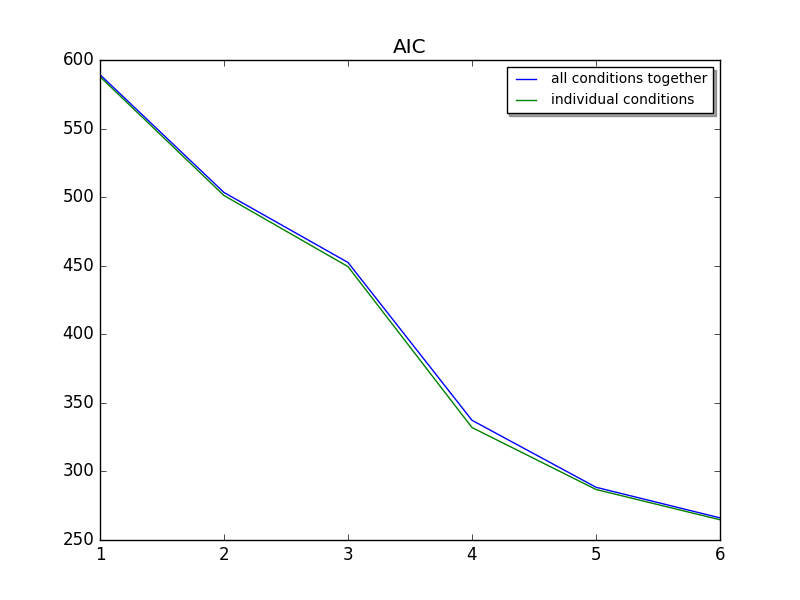
\includegraphics[width=.8\linewidth]{../images/aic_better}  

		\caption{AIC}
		\label{fig:AIC}

	\end{minipage}
	\quad
	\begin{minipage}[b]{0.33\linewidth}
		\centering
		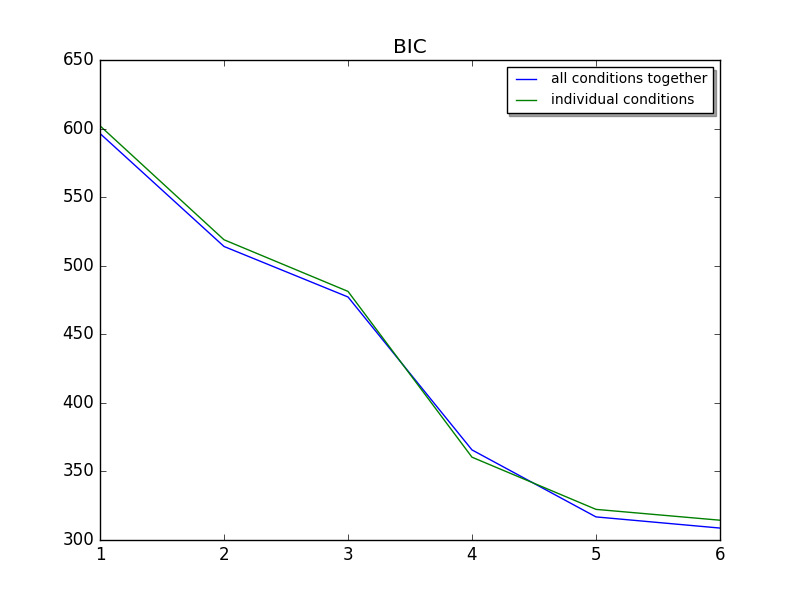
\includegraphics[width=.8\linewidth]{../images/bic_better}  
		\caption{BIC}
		\label{fig:BIC}

	\end{minipage}
		
	\begin{minipage}[b]{0.33\linewidth}
		\centering
		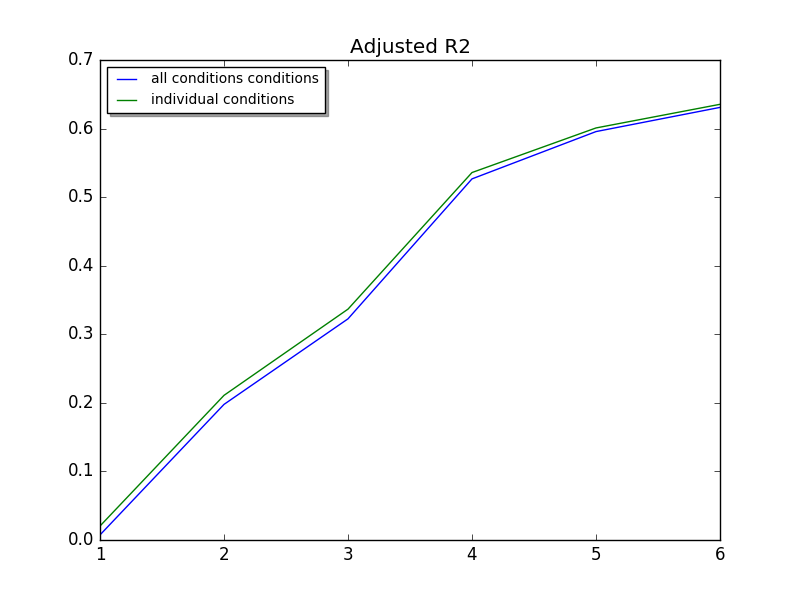
\includegraphics[width=.8\linewidth]{../images/adjr2_better}  
		\caption{Adjusted $R^2$}
		\label{fig:adjr2}

	\end{minipage}

\end{figure}

	

